\documentclass[11pt, a4paper]{article}

\usepackage[utf8]{inputenc}
\usepackage[greek, english]{babel}
\usepackage{alphabeta}
\usepackage{libertine}
\usepackage{graphicx}
\usepackage{biblatex}[sorting=nty] % sort alphabetically
\usepackage[table]{xcolor}
\usepackage{mathptmx} % Times New Roman
\usepackage{makecell}
\usepackage{setspace}
\usepackage{geometry}

\pagenumbering{arabic}
\onehalfspacing % Set line spacing to 1.5
\graphicspath{ {./results/} }
\addbibresource{refs.bib}

\def\code#1{\texttt{#1}}

\title{\Huge Supplemental Material Part 1: Crawled Data Analysis\\
	\LARGE Practical Data Science: 2nd Project}

\author{\Large  Tsirmpas Dimitris }


\begin{document}
	
	\maketitle
	\begin{center}
		\large Athens University of Economics and Business \\
		\large MSc in Data Science
		
	\end{center}
	
	
	\section{Introduction}
	This report outlines results and conclusions drawn from the mechanical annotation of Greek and Greeklish YouTube comment data. The full report, detailing goals, data sources, methodology and implementation can be found at \url{https://github.com/dimits-exe/practical_data_science}.
	
	Our operational data have been collected by the top results of YouTube search for two categories: \textbf{Greek songs} and \textbf{Greek Gaming videos}. These categories represent two main demographics of the Greek online community: The older, middle-aged and the younger generations.
	
	
	\section{Language Identification Results}
	
	The main questions about our dataset are:
	\begin{itemize}
		\item How often is Greeklish spoken in circles of young and old people?
		\item How much do Greek and English users use emojis in comments?
		\item Do comments in Greeklish use emojis more often than comments in Greek?
		\item Is there any trend towards using Greeklish in the recent years?
	\end{itemize}
	
	Below, we present supporting graphs.
	
	
	
	\begin{figure}[h!]
		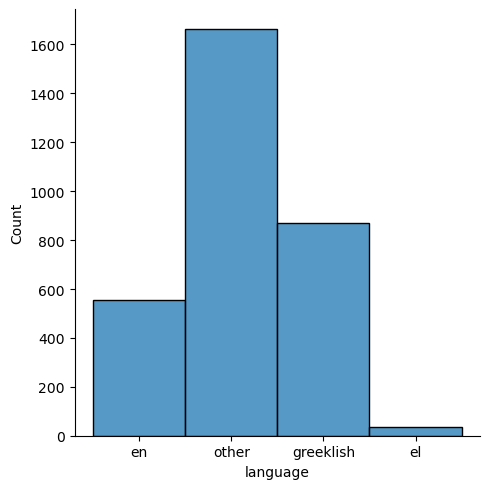
\includegraphics[width=8cm]{lang_dis.png}
		\centering
		\caption{Language distribution in the crawled dataset.}
		\label{fig::lang_dis}
	\end{figure}
	
	\begin{figure}[h!]
		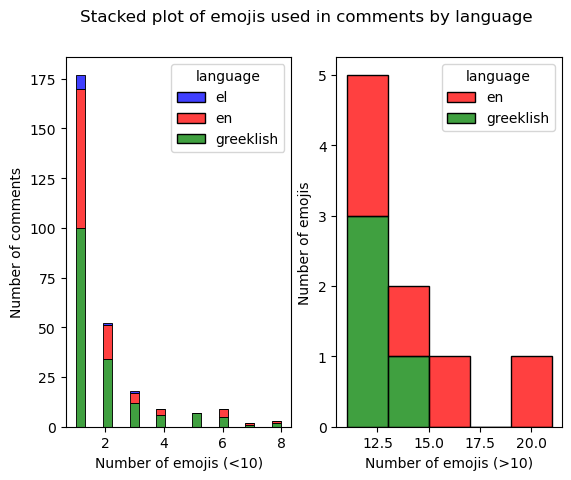
\includegraphics[width=8cm]{emojis_dis.png}
		\centering
		\caption{Stacked plot of emoji usage by language.}
		\label{fig::emojis_dist}
	\end{figure}
	
	\begin{figure}[h!]
		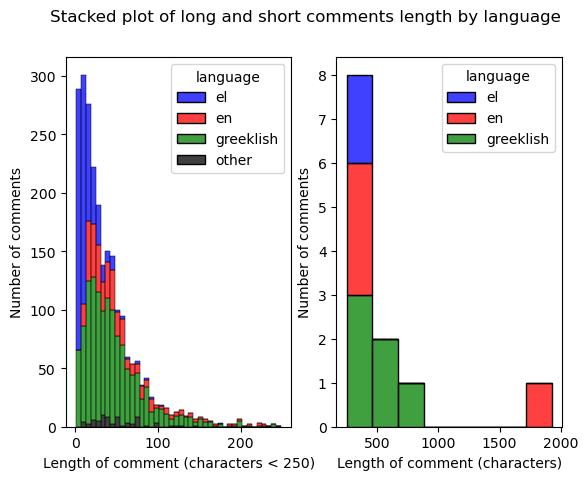
\includegraphics[width=8cm]{length_dis.png}
		\centering
		\caption{Length of comments by language, measured by characters.}
		\label{fig:length_dis}
	\end{figure}
	
	\begin{figure}[h!]
		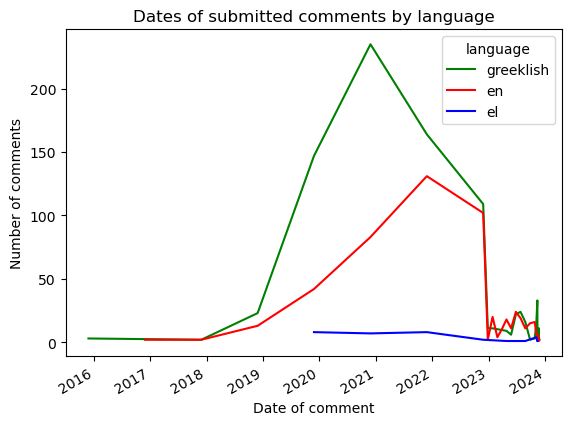
\includegraphics[width=8cm]{time_plot.png}
		\centering
		\caption{Number of comments by language for each day, running from 2017 to present.}
		\label{fig::timeseries.png}
	\end{figure}
	
	
	
	\section{Toxicity Classification Results}
	
	
\end{document}